%% ================================================================================
%% Reuniwatt document latex template                                     
%%                                   
%% ================================================================================

\documentclass[a4paper,12pt]{article}
%\usepackage[latin1]{inputenc}
\usepackage[T1]{fontenc}
\usepackage[utf8]{inputenc}
\usepackage{calc}
\usepackage{setspace}
%\usepackage{fixltx2e}
\usepackage{graphicx}
\usepackage{multicol}
\usepackage{textcomp} %to avoid a warning generated by gensymb
\usepackage{gensymb}
\usepackage[normalem]{ulem}
%% Please revise the following command, if your babel
%% package does not support fr-CA
%\usepackage[frenchb]{babel}
\usepackage[round,authoryear,sort&compress]{natbib}
\usepackage[UKenglish]{babel}
\usepackage{caption}
%\usepackage{subcaption} %cannot be used together with subfig!
\usepackage{color}
\usepackage{hyperref}

\usepackage{eurosym}
\usepackage{lastpage}
\usepackage{vhistory}
%\usepackage[style=authoryear,natbib=true,maxcitenames=1]{biblatex}
\usepackage{amsmath, amsthm, amssymb, amsfonts}
\usepackage{xurl} %added by FK

\usepackage{coverpage_reuniwatt}
\usepackage{multirow}

\newcommand\MyBox[2]{
  \fbox{\lower0.75cm
    \vbox to 1.7cm{\vfil
      \hbox to 1.7cm{\hfil\parbox{1.4cm}{#1\\#2}\hfil}
      \vfil}%
  }%
}
  
\usepackage[
  top=2cm,
  bottom=3cm,
  left=3cm,
  right=3cm,
  headheight=33.33pt, % as per the warning by fancyhdr
  headsep=2cm,
  includehead,includefoot,
  heightrounded, % to avoid spurious underfull messages
]{geometry} 
  
  
%Reuniwatt header and footer
\usepackage{fancyhdr}
\pagestyle{fancy}
\fancyhf{}
\renewcommand\headrule{}
\renewcommand{\footrulewidth}{1pt}
\renewcommand{\footrule}{\hbox to\headwidth{\color{red}\leaders\hrule height \headrulewidth\hfill}}

\fancyfoot[CE,CO]{\footnotesize Reuniwatt SAS, 14 rue de la Guadeloupe, 97490 Sainte-Clotilde\\
Tel : 06.92.64.43.13 / Fax : 02.62.92.10.20 / courriel : info@reuniwatt.com\\
Soci\'{e}t\'{e} par Actions Simplifi\'{e}e au capital de 191.700\euro\ RCS Saint-Denis 518 919 345}

\rhead{Page \thepage/\pageref{LastPage}}
\lhead{
\includegraphics[scale=0.2]{reuniwatt.jpg}}


%\renewcommand \vhChangeColWidth{1.2\hsize}
%\renewcommand \vhAuthorColWidth{2\hsize}

%titre
\title{Title: The Reuniwatt LaTeX Template}

\hyphenation{Re-uni-watt Bar-quiss-eau Ra-dio-sound-ing} %custom hyphenation list
\setlength\parindent{0pt} %FK edit: no indent at beginning of paragraph
 
\begin{document}
\hbadness=10000  %FK edit: less warnings for underfull/overfull hboxes

\maketitle
\addtocounter{page}{1}

% Start of the revision history table   
\begin{versionhistory}
  \vhEntry{1.0}{13.10.2017}{LEB}{Created template.}
  \vhEntry{1.1}{23.03.2021}{FK}{Edits in template.}
  \vhEntry{1.2}{24.03.2021}{FK}{This revision history is part of the template. Please use it.}
  %\vhEntry{1.1}{}{}{}
\end{versionhistory}
\setcounter{table}{0}
\newpage
\tableofcontents
\newpage

\section*{Purpose of the document}
\addcontentsline{toc}{section}{Purpose of the document}

The purpose of this document is to show you what the Reuniwatt LaTeX template looks like. Have fun editing! In your own documents, please use this section to explain the purpose of your document.

\newpage

\section{Hyphenation}

If latex does not know a word, it would not know how to line break it properly, which will lead to a warning. A file for hyphenation is loaded above. It includes information on where latex can break words.

\section{Tables and figures}

\subsection{Static table}

Table~\ref{tab:model_levels} shows an example of a simple table.

\begin{table}[!htb]
  \centering
  \begin{tabular}{cc}
  \hline
  \hline
  Model level & Altitude (m)  \\ \hline
  137 & 10.00 \\
  \hline
  136 & 30.96 \\
  \hline
  135 & 53.92 \\
  \hline
  134 & 79.04 \\
  \hline
  133 & 106.54 \\
  \hline
  132 & 136.62 \\
  \hline
  \hline
  \end{tabular}
  \caption{First levels of the ECMWF model.}
  \label{tab:model_levels}
\end{table}

\subsection{Dynamic table}

Table~\ref{tab:workpackages} gives an example of a table that adjusts the font size depending on the content.

\begin{table}[!htb]
  \tiny
  \begin{tabular}{lllll}
    \begin{tabularx}{\textwidth}{|X|X|l|l|}
      \hline
      Work package reference                                                                           & Work package name in work plan                                            & MM/YYYY & Responsible \\ \hline
\begin{tabular}[c]{@{}l@{}}[Work package 1] - For me\\ Preparation algorithms\end{tabular}                & Preparation \& of the amazing algorithm I want to develop                     & 08/2020 & Me                     \\ \hline
\begin{tabular}[c]{@{}l@{}}[Work package 2] - For you\\ Testing algorithms\end{tabular}                & Experimental implementation of the algorithm                                   & 09/2020 & You                     \\ \hline
\begin{tabular}[c]{@{}l@{}}[Work package 3] - For us\\ Validating algorithms\end{tabular}                & Validation of the amazing algorithm with reference data                    & 10/2020 & All of us                     \\ \hline
    \end{tabularx}
  \end{tabular}
  \caption{Work packages related to the development of the amazing algorithm.}
  \label{tab:workpackages}
\end{table}

\subsection{A figure}

Figure~\ref{fig:turbinegrowth} shows an example of a figure.

\begin{figure}[!htb]
  \centering
  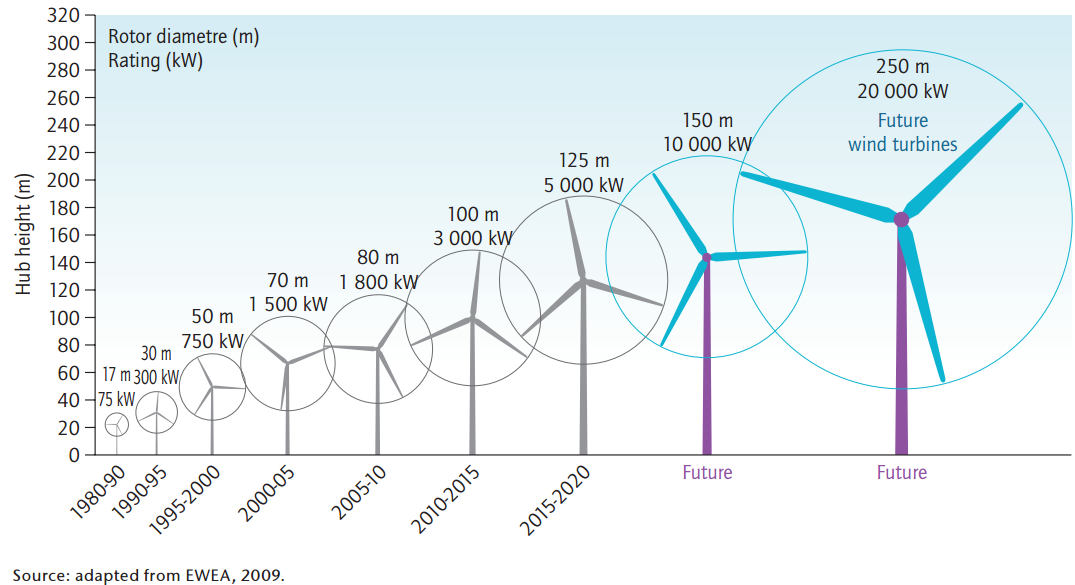
\includegraphics[width=0.9\textwidth]{figures/TurbineGrowth.png}
  \caption{Growing size of wind turbines since 1980 and perspectives. Sources: IEA, EWEA.}
  \label{fig:turbinegrowth}
\end{figure}

\section{Equations}

Equation~\ref{eq:rmse} is a lovely equation.

\begin{equation}
  RMSE=\sqrt{\frac{\sum_{i=1}^{n} (\hat{y}_i - y_i)}{n}}
  \label{eq:rmse}
\end{equation}

\section{Citations}

The file ReuniwattPublications.bib contains all publications of Reuniwatt until beginning of 2021. It contains classics such as \cite{diagne_review_2013}, an early review paper of Reuniwatt that has been cited hundreds of times. The bib file has been exported directly from Zotero. Ask Frederik if you want to know more about that. To cite a paper within a sentence you can do it like this \cite{liandrat_comparison_2021}. Citing a paper at the end of a sentence works like this \citep{roussel_cloud_2019}.

\newpage

\section{Weblinks}

Sometimes links are very long and do not fit into one line, such as \url{https://reuniwatt.com/en/2021/02/02/webinar-series-intelligent-camera-cloud-operators-for-numerical-weather-prediction/}. The package xurl allows to line break them automatically.

\bibliographystyle{abbrvnat}
\bibliography{ReuniwattPublications}

\end{document}